\begin{center}
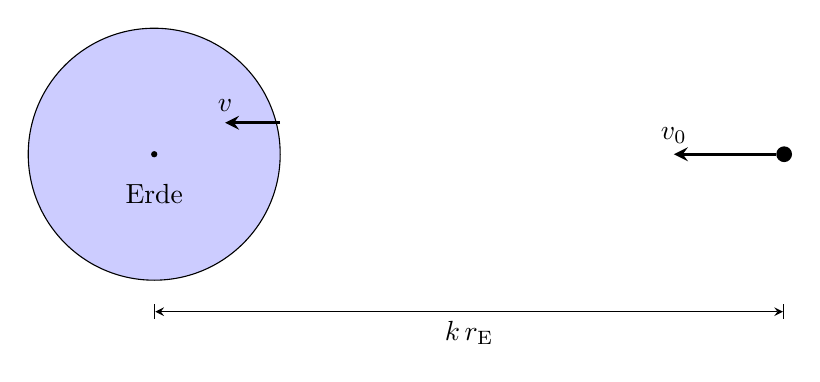
\begin{tikzpicture}[>=stealth]
 \fill[blue!20] (0,0) circle (1.6);
 \draw (0,0) circle (1.6);
 \fill (0,0) circle (0.04);
 \node at (0,-0.5) {Erde};

 \fill (8,0) circle (0.1);
 \draw[->, very thick] (7.9,0) -- (6.6,0) node[above] {$v_0$};
 \draw[|<->|] (0,-2) -- (8,-2) node[midway, below] {$k\,r_\mathrm{E}$};
 \draw[->, very thick] (1.6,0.4) -- (0.9,0.4) node[above] {$v$};
\end{tikzpicture}
\end{center}

Die Entfernung wird vom Erdmittelpunkt aus gemessen: $r_0 = k\,r_\mathrm{E}$ mit $k = \kMO$. Ohne Luftwiderstand bleibt die Summe aus kinetischer Energie und Gravitationsenergie erhalten:
\begin{align}
 \frac{1}{2}\,m\,v_0^2-G\,\frac{M_\mathrm{E}\,m}{k\,r_\mathrm{E}} &= \frac{1}{2}\,m\,v^2-G\,\frac{M_\mathrm{E}\,m}{r_\mathrm{E}}
\end{align}
Aufgelöst nach der Aufprallgeschwindigkeit:
\begin{align}
 v &= \vEnF \\
   &= \sqrt{\left(\vA\right)^2+2\cdot\frac{\ncG\cdot\MEr}{\REr}\cdot\left(1-\frac{1}{\kMO}\right)} \\
   &= \vEn \approx \result{\vEnP{3}{2}}
\end{align}
mit $M_\mathrm{E} = \MErO$ und $r_\mathrm{E} = \RErO$ (FoTaBe S.~209).
